% core TikZ only; no extra library beyond the paper preamble is required.
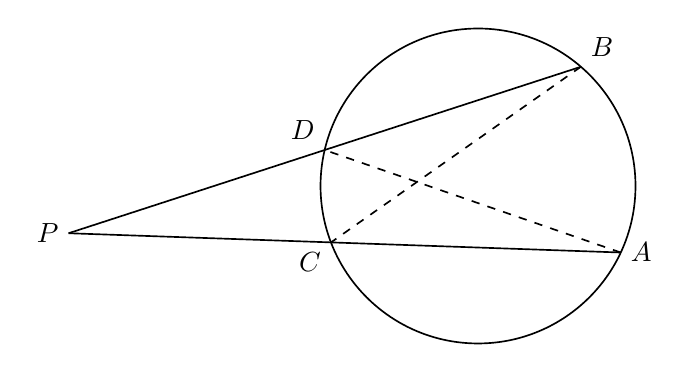
\begin{tikzpicture}[x=1cm,y=1cm,line width=.6pt,font=\normalsize]
\coordinate (P) at (0,0);
\coordinate (O) at (5.2,0.6);
\coordinate (D) at (3.252896,1.05693);
\coordinate (B) at (6.506664,2.114143);
\coordinate (C) at (3.332703,-0.116381);
\coordinate (A) at (7.012776,-0.244892);
\draw (O) circle[radius=2cm];
\draw (P)--(B);
\draw (P)--(A);
\draw[dashed] (A)--(D);
\draw[dashed] (B)--(C);
\node[left] at (P) {$P$};
\node[above left] at (D) {$D$};
\node[above right] at (B) {$B$};
\node[below left] at (C) {$C$};
\node[right] at (A) {$A$};
\end{tikzpicture}
